\section{Patterns 4 - State patterns}

\subsection{Fokuspunkter}

\begin{itemize}
	\item Redegør for, hvad et software design pattern er.
	%\item Redegør for de forskellige måder at implementere en state machine på.
	\item Redegør for strukturen i GoF State Pattern.
	\item Sammenlign  switch/case-implementering med GoF State.
	\item Redegør for fordele og ulemper ved anvendelsen af GoF State.
	\item Redegør for, hvordan et UML (SysML) state machine diagram mapper til GoF State.
\end{itemize}

\subsection{Hvad er et Software pattern?}

\derp

\subsection{Redegør for strukturen i et state pattern}
Et state pattern er et behavioral pattern, og er en måde at implementere en state machine på.

State mønstret definerer en mpde hvorpå vi kan ændre et objekts opførsel eftersom dens interne state ændres (run-time).
State mønstret giver mulighed for at implementere store forskelle i opførslen uden brug af masser af Switches of if sætninger.

\begin{figure}[h]
\centering
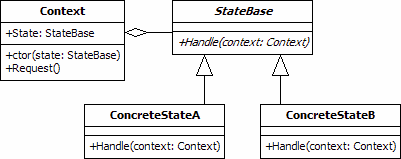
\includegraphics[width=0.5\linewidth]{figs/state/gofState}
\caption{UML for et GoF state pattern}
\label{fig:gofState}
\end{figure}

\begin{enumerate}
	\item Context klassen - Definerer et interface der bruges af klienter. Indeholder en instans af en ConreteState subclass, der kan definere en Current State.
	\item StateBase klassen - Et interface til indkapsling af ConcreteStates adfærd
	\item Concrete State - Hver ConcreteState implementerer den adfærd der associeres til i Context klassen.
\end{enumerate}

\subsubsection{Kodeeksempel}

Dette er et kodeekspempel på en state machine der kan toggle dens state.

\begin{lstlisting}[caption=StateBase klassen]
abstract class State
{
	public abstract void Handle(Context context);
}
\end{lstlisting}

Som det ses på klassen StateBase implementering, har den blot en abstrakt metode der tager mod en Context

\begin{lstlisting}[caption=ConcreteStateA klassen - Switcher til State B]
class ConcreteStateA
{
	public override void Handle(Context context)
	{
		context.State = new ConcreteStateB;
	}
}
\end{lstlisting}

\begin{lstlisting}[caption=StateBase klassen - Switcher til state A]
class ConcreteStateB
{
	public override void Handle(Context context)
	{
		context.State = new ConcreteStateA;
	}
}
\end{lstlisting}


\begin{lstlisting}[caption=Context klassen - Bruges i main() til at kalde Request()]
  class Context
  {
	  private State _state;
  
	  // Constructor
	  public Context(State state)
	  {
		  this.State = state;
	  }
  
	  // Gets or sets the state
	  public State State
	  {
		  get { return _state; }
		  set
	   {
	  
		   _state = value;
		   Console.WriteLine("State: " +
		   _state.GetType().Name);
	   }
	  }
  
	  public void Request()
	  {
		  _state.Handle(this);
	  }
  }
\end{lstlisting}
\newpage

I lærebogen erklæres alle states static inde i contexten idet der således ikke skal laves en ny, hver gang der skiftes state... Smart.


\paragraph{State vs. Strategy.}
Ser man på UML'en for et State Pattern, ligner det jo et strategy pattern. I et State  pattern eksisterer der dog et constraint idet hver ConcreteState klasse skal bruge en reference til en Context (den vælger og invoker contextens metoder igennem denne reference). Dette constraint eksisterer ikke i et strategy pattern:

\begin{lstlisting}[caption=Klients brug af strategy pattern]
IStrategy myStrategy = new s1();
myStrategy .StragetyFunction();

myStrategy = new s2();
myStrategy .StragetyFunction();
\end{lstlisting}


\subsection{Sammenlign switch/case-implementering med GoF State.}


